\section{Example}
\label{sec:example}
In this section, we illustrate the \CodeIn{eXpress} approach with an example. \CodeIn{eXpress} takes as input two versions of a program and produces as output a regression test suite. The test suite on execution detects behavioral differences (if any exist) between the two versions of program under test. Although \CodeIn{eXpress} analyzes assembly code of C\# programs, in this section, we illustrate the \CodeIn{eXpress} approach using program source code. 


\begin{figure}[t]
\Comment{
\begin{tiny}
\begin{alltt}

  \hspace{0.5cm}\textbf{static public int} testMe(\textbf{int }x, \textbf{int[] } y)\{
1 \hspace{1.0cm} \textbf{int} j=1;
2 \hspace{1.0cm} \textbf{if}(x==90)\{
3 \hspace{1.5cm} \textbf{for}(\textbf{int} i=0; i< y.Length; i++)\{
4 \hspace{2.0cm} \textbf{if}(y[i] == 15)
5 \hspace{2.5cm} x++;
6 \hspace{2.0cm} \textbf{if}(y[i] == 16)
7 \hspace{2.5cm} j=2;
8 \hspace{2.0cm} \textbf{if}(y[i] == 25)
9 \hspace{2.5cm} \textbf{return} x;
10\hspace{2.0cm} \textbf{if}(x == 110)
11\hspace{2.5cm} x = j+2; //x = 2*j+1
12\hspace{2.0cm} \textbf{if}(x>110) 
13\hspace{2.5cm} \textbf{return} x;
14\hspace{1.5cm} \}
15\hspace{1.0cm} \}
16\hspace{1.0cm} \textbf{return} x;
  \hspace{0.5cm}\}
 
\end{alltt}
\end{tiny}
}


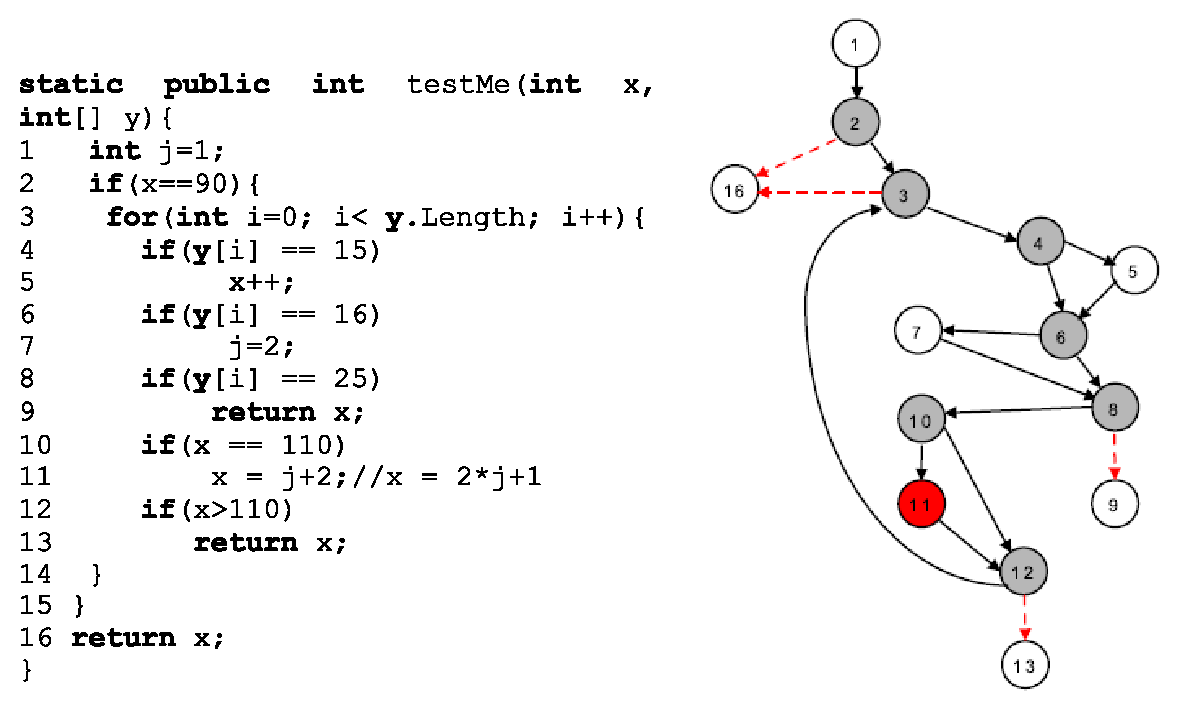
\includegraphics[width=8cm, keepaspectratio]{Figures/examp}
\vspace{-0.25 in}
\caption{An example program}
\vspace{-0.2 in}
\label{fig:example}
\end{figure}

	Consider the example in Figure~\ref{fig:example}. Suppose that the statement at Line 11 of \CodeIn{testMe} has been modified resulting in the one shown in the comment at Line 11.
	The \CodeIn{Difference Finder} component of \CodeIn{eXpress} compares the original and the new versions of the program under test to find differences between each corresponding method of the two program versions. For the program in Figure~\ref{fig:example}, \CodeIn{Difference Finder} detects that the statement at Line 11 is changed in the new version. The \CodeIn{Graph Builder} component of \CodeIn{eXpress} then builds a Control-Flow Graph (CFG) of the new version of  the program under test and marks the changed vertices in the graph. Figure~\ref{fig:example} also shows the CFG of the example program. The labels of vertices in the CFG show the corresponding line numbers in Figure~\ref{fig:example}. The red (dark) vertex shows the changed statement at Line 11. The \CodeIn{Graph Traverser} component traverses the CFG to find all the branches\footnote{\scriptsize{A branch is an outgoing edge of a branching node}} $b$ in a program such that if $b$ is taken, the program execution cannot reach the dark vertex at Line 11. 
	\Comment{
	For each branch $b$ in the program, the \CodeIn{Graph Traversal} component tries to find a path from the source vertex of $b$ to the dark vertex with $b$ as the first edge in the path.	For each vertex in the graph with a degree\footnote{\scriptsize{The degree of a vertex in a graph is the number of edges starting from the vertex. The nodes having a degree greater than one}} of more than one (the vertices colored gray), the \CodeIn{Graph Traversal} component tries to find a path from a gray vertex to the dark vertex through each branch (edge) of the gray vertex.
	For example, \CodeIn{Graph Traverser} tries to find a path between the gray vertex labeled 8 in Figure~\ref{fig:CFG} and the dark vertex labeled \ref{fig:CFG} through both of the edges $<8, 9>$ and $<8, 10>$. \CodeIn{Graph Traverser} finds a path $<8, 10, 11>$ through branch $<8,10>$ but is not able to find any path through the branch <8,10>.
	}On traversing the CFG in Figure~\ref{fig:example}, the \CodeIn{Graph Traversal} detects that taking the branches $<2, 16>$, $<3, 16>$, $<8, 9>$, and $<12, 13>$ (dotted/dark red edges in Figure~\ref{fig:example}), the program execution cannot reach the vertex at Line 11. Hence, the execution of these branches cannot help in executing the statement at Line 11; behavioral differences between two versions of the program cannot be detected without executing the changed statement at Line 11. Hence, these branches are not explored by the \CodeIn{Dynamic Test Generator} component of \CodeIn{eXpress} while generating regression tests for the program under test. 
\Comment{
	\begin{figure}[t]
    \centering
        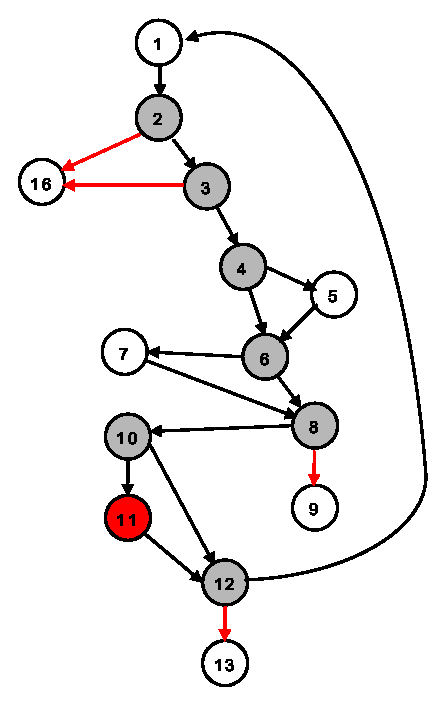
\includegraphics[width=3cm, keepaspectratio]{Figures/exampleCFG2}
    \caption{Control-Flow Graph for the program in Figure~\ref{fig:example}}
    \vspace{-0.2 in}
    \label{fig:CFG}
    \vspace{-0.2 in}
\end{figure}
}

The \CodeIn{Instrumenter} component transforms the two versions of the
program code such that the transformed program code is
amenable to regression testing. In particular, the \CodeIn{Instrumenter} component
instruments both versions of the program under test. The
instrumentation allows us to compare the internal behavior
of running the same generated test on the two versions.
	
	Figure~\ref{fig:Changed} shows the code of \CodeIn{testMe}'s new version after instrumentation. The \CodeIn{Instrumenter} component inserts a statement (Line 12 in Figure~\ref{fig:Changed}) just after any changed	 statement (Line 11 in Figure~\ref{fig:example}). The instrumented statement allows us to store the current value of \CodeIn{x} in a particular run $r$ (i.e., an explored path) of DSE. In particular, this statement results in an assertion \CodeIn{PexAssert.IsTrue ("uniqueName", x == currentX)}\footnote{\scriptsize{\CodeIn{PexAssert} is an API class provided by Pex.}} in the test generated in run $r$, where \CodeIn{currentX} is the value of $x$ at Line 12 in the new version of the program. One such assertion is added by Pex to the generated test each time the statement is executed in the loop. Hence, if the loop containing the changed statement executes 20 times, 20 such assertions will be added to the test generated by Pex.
The generated test can be executed on the original version of \CodeIn{testMe} to compare program states at Line 12 after the execution of the changed statement with the ones captured in the execution of the new version. 
			
\begin{figure}[t]
\begin{tiny}
\begin{alltt}
  \hspace{0.5cm}\textbf{public boolean} testMe(\textbf{int }x, \textbf{int[] } y)\{
  \hspace{1.0cm} ...
10\hspace{1.0cm} \textbf{if}(x == 110)\{	 
11\hspace{1.5cm} x = 2*j+1;
12\hspace{1.5cm} \textbf{PexStore.ValueForValidation}("uniqueName", x);
13\hspace{1.0cm} \} 
  \hspace{1.0cm} ...
  \}
\end{alltt}
\end{tiny}
\vspace{-0.2 in}
\caption{\scriptsize{Instrumented example program after instrumentation}}
\label{fig:Changed}
\vspace{-0.25 in}
\end{figure}

If there are multiple changed statements in the program, our approach first finds multiple regions each of which contains nearby changed statements in the program. We refer to each of such regions as a changed region\footnote{\scriptsize{A changed region is a minimal set of statements that contains all the changed statements in a method. There can be a maximum of one region per method.}} in the rest of the paper. Our approach finds all the variables and fields that are identified as defined in a changed region and inserts statements (such as the statement at Line 12 of Figure \ref{fig:Changed}) to log the value of each defined variable or field in the changed region. If a defined variable is a non-primitive type, such a statement enables to compare program states by comparing the object graphs reachable from the logged values. The \CodeIn{Dynamic Test Generator} component of \CodeIn{eXpress} then performs DSE on the instrumented new version of the program to generate regression tests. 

\CodeIn{eXpress} performs DSE on the instrumented new version of the program. After each run of DSE, \CodeIn{eXpress} executes the generated test on the instrumented original version (in the same way as instrumentation of the new version) to check whether the program state is infected after the execution of a changed region. The instrumentation enables us to perform only one instance of DSE on the new version instead of performing two instances of DSE: one on the original and the other on the new program version. Performing two instances of DSE can be technically challenging since we have to perform the two DSE instances in a controlled manner such that both versions are executed  with the same input and the execution trace is monitored for both the versions by a common exploration strategy to decide which branching node to flip next in the two versions. 

The \CodeIn{Dynamic Test Generator} component of \CodeIn{eXpress} uses Dynamic Symbolic Execution (DSE) to generate tests for the new version. DSE iteratively generates test inputs to cover various feasible paths in the program under test. In particular, DSE flips some branching node from a previous execution to generate a test input for covering a new path. The node to be flipped is decided by a search strategy (also called exploration strategy) such as depth-first search. \CodeIn{Dynamic Test Generator} implements a search strategy for Pex~\cite{Pex} to efficiently find behavioral differences between two versions of a program.

To cover the changed statement at Line 11, DSE needs inputs
$x=90$ and the array $y$ of length greater than 20 where at least 20 elements of y
have a value 15 and no element has a value 25. To generate the input, DSE needs to execute the loop at least 20 times. In each iteration DSE has the choice of flipping branching nodes at Lines 4, 6, 8, 10, 12, a search space of $2^{100}$ paths (considering a loop bound of 20). 
  
To reduce the branch search space of DSE, the \CodeIn{Dynamic Test Generator} component adopts the PIE model~\cite{voas} of error propagation described in Section~\ref{sec:intro}. In particular, the \CodeIn{Dynamic Test Generator} prunes all the following branches from the search space of DSE.
\\ \textbf{Branches not satisfying E}. The branches $<2, 16>$, $<3, 16>$, $<8, 9>$, and $<12, 13>$ found to be irrelevant by the \CodeIn{Graph Traverser} component cannot help in executing the changed statement at Line 11. Hence, these branches are not explored by the \CodeIn{Dynamic Test Generator} component. 
\\ \textbf{Branches not satisfying I}. Suppose
that we cover the changed statement at Line 11 in Figure 1 using inputs
$x=90$ and the array $y$ of length $20$ where each element of $y$
has a value $15$. The execution takes a path $P$ executing the
loop $20$ times, assigning the variable $x$ to $110$ and eventually
covering the changed statement at Line 11 . However, the program state after the
execution of  changed statement is not infected since after the first execution
of the changed statement, the value of $x$ is $3$ in both versions. In such situations, the branching nodes in the execution path
that are after the last instance of the changed node are not explored. For the example, the branch $<12, 3>$ is pruned from exploration.
\Comment{
\item \textbf{Branches not satisfying P}. Suppose the changed statement is executed, the program
state is infected after the execution of the changed statement, but the infection
does not propagate to an observable output.  We do
not explore the branches after the execution of the changed statement if these
branches do not lead to any other changed region.
}
\Comment{
For the example in Figure~\ref{fig:example}, our approach takes ** DSE runs to execute the changed statement, while the default strategy in Pex~\cite{Pex} takes ** DSE runs. To infect the program state, our approach takes ** DSE runs. The program state was propagated as soon as it was infected.
		}






\Comment{
\begin{figure}[t]
\begin{CodeOut}
\begin{alltt}
  [PexFactoryClass]
  \textbf{public class} FactoryClass\{
  \hspace{0.5cm}[PexFactoryMethod(typeof(\textbf{TestClassSynthesized}))]
  \hspace{0.5cm}\textbf{public static TestClassSynthesized} create(int a, 
  \hspace{1.5cm}int b, int c, int n)\{
  \hspace{1.0cm}\textbf{TestClassSynthesized} obj = 
  \hspace{1.5cm}\textbf{new} TestClassSynthesized(); 
  \hspace{1.0cm} \textbf{for}(int i=0; i< methodSeuenceLength; i++)\{
  \hspace{1.5cm} \textbf{switch}(n)
  \hspace{2.0cm} \textbf{case} 0: \textbf{obj}.A(a);\textbf{break};
  \hspace{2.0cm} \textbf{case} 1: \textbf{obj}.B(b);\textbf{break};
  \hspace{2.0cm} \textbf{case} 2: \textbf{obj}.C(c);\textbf{break};
  \hspace{2.0cm} \textbf{case} 3: \textbf{obj}.testMe();\textbf{break};
  \hspace{2.0cm} \textbf{default}: \textbf{break};
  \hspace{1.0cm}\}
  \hspace{1.5cm} \textbf{return} obj;
  \hspace{0.5cm}\}
  \}
\end{alltt}
\end{CodeOut}
\caption{Factory Class to generate an object of \CodeIn{TestClassSynthesized}}
\label{fig:factory}
\end{figure}
}




\Comment{
In this section, we illustrate our approach with the aid of an example. Our approach takes as input two versions of a class and produces as output a regression test suite. The test suite on execution detects behavioral differences between the two versions of class under test. Our approach is inspired by the PIE model~\cite{voas} of error propagation. According to the PIE model, a fault can be detected by a test suite if the fault is executed (E), the execution of the fault infects the state (I), and that the infected state propagates to the output (P). We have implemented our approach in Pex~\cite{Pex}, an automated structural testing tool based on for .NET developed at Microsoft Research. Pex uses Dynamic Symbolic Execution (DSE)~\cite{dart, cute} to explore various paths in the program and generate a unique test for each feasible path explored. To make the DSE efficiently in finding behavioral differences, our approach guides the DSE to avoid exploring irrelevant paths that cannot help in achieving E, I, or P of the PIE model.

\begin{figure}[t]
\begin{CodeOut}
\begin{alltt}
  \textbf{public} TestClass\{
  \hspace{0.5cm}\textbf{public boolean} testMe(\textbf{int }x, \textbf{int[] } y)\{
1 \hspace{1.0cm} \textbf{int} j=0, k=0;
2 \hspace{1.0cm} \textbf{if}(x==90)\{
3 \hspace{1.5cm} \textbf{for}(\textbf{int} i=0; i< y.Length; i++)\{
4 \hspace{2.0cm} \textbf{if}(y[i] == 15)
5 \hspace{2.5cm} x++;
6 \hspace{2.0cm} \textbf{else if}(y[i] == 25)
7 \hspace{2.5cm} \textbf{return} x;
8 \hspace{2.0cm} \textbf{if}(x >= 110 && x<= 150)
9 \hspace{2.5cm} j =1;
10\hspace{2.0cm} \textbf{else if}(x>150)
11\hspace{2.5cm} j =2;
12\hspace{2.0cm} \textbf{for}(i=200; i<= x; i++)
13\hspace{2.5cm} k++;
14\hspace{2.0cm} \textbf{if}(j > 0) // \textbf{if}(j >= 0)
15\hspace{2.5cm} x = j+2; //x = 2*j+1
16\hspace{2.0cm} \textbf{for}(int i=0; i< k+1; i++) 
17\hspace{2.5cm} x = x*k;
18\hspace{1.5cm} \}
19\hspace{1.0cm} \}
20\hspace{1.0cm} \textbf{return} x;
  \hspace{0.5cm}\}
  \hspace{0.5cm}...
  \hspace{0.5cm}A (\textbf{a})...
  \hspace{0.5cm}B (\textbf{b})...
  \hspace{0.5cm}C (\textbf{c})...
  \}  
\end{alltt}
\end{CodeOut}
\vspace{-0.15 in}
\caption{An Example Program}
\vspace{-0.55 in}
\label{fig:example}
\end{figure}


Consider the example in Figure~\ref{fig:example}. Figure~\ref{fig:example} contains a class \CodeIn{TestClass}. The class \CodeIn{TestClass} contains a method \CodeIn{testMe} that has been changed in the new version. The class also contains 3 other methods \CodeIn{A}, \CodeIn{B}, and \CodeIn{C} that have not been changed in the new version. Suppose the statement at Line 15 of the method \CodeIn{testMe} has been modified to the one shown in the comment at Line 15. Our approach first constructs the control flow graph for the two versions and finds differences between the two control flow graphs. Our approach detects that Line 14 in the program has been changed. Instead of performing DSE separately for each version, our approach synthesizes a new class combining the two program versions as shown in Figure~\ref{fig:Changed}. As shown in Figure~\ref{fig:Changed}, our approach inserts an argument \CodeIn{isOriginalVersion} of type \CodeIn{boolean} in the method containing the changed statement. Our approach also inserts new branches at the location of changed statement(s). The \CodeIn{true} branch contains the original statement while the \CodeIn{false} branch contains the modified statement. The \CodeIn{true} branch is executed when \CodeIn{isOriginalVersion} is \CodeIn{true} and vice versa. The Line 15 in Figure~\ref{fig:example} has been changed to Lines 15-18 in Figure~\ref{fig:Changed}. The \CodeIn{true} branch of the \CodeIn{if} statement contains the original statement, while the false branch contains the statement in new version. The synthesized class \CodeIn{TestClassSynthesized} helps us in concurrently running the two versions without having to execute two instances of DSE on the two versions. After every run of DSE, we flip the \CodeIn{if(isOriginalVersion)} branch (if the branch is executed in that particular run) to check the program behavior in the new version. In the rest of this section we will refer to the program in Figure~\ref{fig:example}. Whenever we refer to comparison of program states after execution of the two versions under test, it means we flip the branch at Line 14 to execute the statement in the other version and compare the program states before and after flipping the branch. 

\begin{figure}[t]
\begin{CodeOut}
\begin{alltt}
  \textbf{public} TestClassSynthesized\{
  \hspace{0.5cm}\textbf{public boolean} testMe(\textbf{int }x, \textbf{int[] } y, 
  \hspace{3cm}\textbf{boolean} isOriginalVersion)\{
  \hspace{2.0cm} ...
14\hspace{2.0cm} \textbf{if}(j > 0)
15\hspace{2.5cm} \textbf{if}(isOriginalVersion)	 
16\hspace{3.0cm} x = j+2;
17\hspace{2.5cm} \textbf{else}
18\hspace{3.0cm} x = 2*j+1
  \hspace{2.0cm} ...
  \}
\end{alltt}
\end{CodeOut}
\vspace{-0.15 in}
\caption{Program synthesized for the example program}
\label{fig:Changed}
\end{figure}

Figure~\ref{fig:PUT} shows a Parameterized Unit Test for pex to generate tests for the method \CodeIn{testMe} in the class \CodeIn{TestClassSynthesized}. Figure~\ref{fig:factory} shows the factory method used for synthesizing an object for \CodeIn{TestClassSynthesized}. The factory method instantiates a new instance of the class \CodeIn{TestClassSynthesized}, generates a sequence of method calls containing all combinations \CodeIn{A}, \CodeIn{B}, \CodeIn{C}, and testMe. The length of the sequence is \CodeIn{methodSeuenceLength} which is set to total number of methods in the class \CodeIn{TestClassSynthesized} (4). 



\begin{figure}[t]
\begin{CodeOut}
\begin{alltt}
  [TestClass]
  \textbf{public class} PUTClass\{
  \hspace{0.5cm}[PexMethod]
  \hspace{0.5cm}\textbf{public boolean} testMePUT(\textbf{TestClassSynthesized} obj, int x, 
  \hspace{1.5cm}int[] y, boolean version)\{
 1\hspace{1.0cm}PexAssume.IsNotNull(obj);
 2\hspace{1.0cm}obj.testMe(x, y, version);
  \hspace{0.5cm}\}
  \}
\end{alltt}
\end{CodeOut}
\vspace{-0.15 in}
\caption{Parameterized test for Method \CodeIn{textMe}}
\label{fig:PUT}
\end{figure}

\begin{figure}[t]
\begin{CodeOut}
\begin{alltt}
  [PexFactoryClass]
  \textbf{public class} FactoryClass\{
  \hspace{0.5cm}[PexFactoryMethod(typeof(\textbf{TestClassSynthesized}))]
  \hspace{0.5cm}\textbf{public static TestClassSynthesized} create(int a, 
  \hspace{1.5cm}int b, int c, int n)\{
  \hspace{1.0cm}\textbf{TestClassSynthesized} obj = 
  \hspace{1.5cm}\textbf{new} TestClassSynthesized(); 
  \hspace{1.0cm} \textbf{for}(int i=0; i< methodSeuenceLength; i++)\{
  \hspace{1.5cm} \textbf{switch}(n)
  \hspace{2.0cm} \textbf{case} 0: \textbf{obj}.A(a);\textbf{break};
  \hspace{2.0cm} \textbf{case} 1: \textbf{obj}.B(b);\textbf{break};
  \hspace{2.0cm} \textbf{case} 2: \textbf{obj}.C(c);\textbf{break};
  \hspace{2.0cm} \textbf{case} 3: \textbf{obj}.testMe();\textbf{break};
  \hspace{2.0cm} \textbf{default}: \textbf{break};
  \hspace{1.0cm}\}
  \hspace{1.5cm} \textbf{return} obj;
  \hspace{0.5cm}\}
  \}
\end{alltt}
\end{CodeOut}
\vspace{-0.15 in}
\caption{Factory Class to generate an object of \CodeIn{TestClassSynthesized}}
\label{fig:factory}
\end{figure}

Our approach works in three phases (1) The Execution Phase (2) The Infection Phase (3) The Propagation Phase . 
\\ \textbf{Execution Phase.} In the Execution Phase, our approach guides the DSE in Pex to execute the changed statement(s) (at Line 15 of Figure~\ref{fig:example}). Our approach first finds all the branches that do not need to be explored for executing the changed statement at Line 15 (of Figure~\ref{fig:example}).  Our approach finds that the branches 6 and 16 (of Figure~\ref{fig:example}) cannot lead to the execution of statement at Line 15 (of Figure~\ref{fig:example}). Hence, our approach prevents Pex from exploring these branch in Execution Phase. 
 
\textbf{Infection Phase. }  The execution of the changed statement does not guarantee the infection of the program state. We compare the program state after the execution of the changed statement in the old and new version of the program under test to detect if the program state is infected. If the program state is not infected after the execution of a changed statement, our approach prevents Pex from exploring the branches after the execution of changed statement. For example, in Figure~\ref{fig:example}, the loop at Line 16 is not explored. 

\textbf{Propagation Phase. } The infected program state does not guarantee that the infection will be propagated to an observation point. We consider the last statement executed in a method as an observation point. All the \CodeIn{return} statements are considered as observation points. If a method does not has any return statement, the observation point is the last statement executed in the program. In this phase, we try to propagate the infection to one observation point at a time.
The method \CodeIn{testMe} in Figure~\ref{fig:example} has 2 observation point at Lines 7 and 20. Since the changed statement is not reachable to he observation point at Line 7, we only consider observation point at Line 20. The program state at an observation point consists of return value and the object fields. We check whether the infected state at Line 15 for the input $I_{63}$ is propagated to the end of program. This is done by comparing the return values and the value of fields after the execution of the return statement at Line 20. Our approach detects that the return value at Line 20 is the same for both versions. Our approach finds the propagation stopping statement by comparing the states after execution of all the statements executed between the changed statement at Line 15 and the return statement at Line 20. Our approach finds that the propagation is stopped after the execution of statement at line 17. The statement at line 17 is now the point of interest. The branches are prioritized based on the data dependence from statement at Line 17. Branches 12 is given the priority score $p=1$, Branch 4 is assigned a priority of score $p=2$, while branch 3 is assigned a score $p=3$. Branch 12 cannot be flipped due to infeasible path condition, hence branch 4 is flipped. The preceding process is continued 50 times until an input is generated that executes the path $P_{113}= 2T, (3T, 4T, 6F, 8F, 10F, 12F, 14F, 16F)^{110},$ $3T, 4T, 6F, 8F, 10T, 12T, 12F, 14T, 16F, 3F$, which results in the propagation of the program infection.
}
\subsection{Incremental Test Generation}
Our approach can reuse an existing
test suite for the original version so that changed parts of the program can be explored
efficiently due to which test generation is likely to find behavior
differences earlier in path exploration. Figure~\ref{fig:example2} shows the new version of a program \CodeIn{testMe}. Suppose that statements at Lines 12 and 13 are added in the new version. 
\Comment{
\begin{figure}[t]
\begin{tiny}
\begin{alltt}

  \hspace{0.5cm}\textbf{static public int} testMe(\textbf{string[] }c)\{
1 \hspace{1.0cm} \textbf{int} state = 0;
2 \hspace{1.5cm} \textbf{for}(\textbf{int} i=0; i< c.Length; i++)\{
3 \hspace{2.0cm} \textbf{if}(c[i] == '[')
4 \hspace{2.5cm} state =1;
5 \hspace{2.0cm} \textbf{if}(state == 1 && c[i] == "\{")
6 \hspace{2.5cm} state =2;
7 \hspace{2.0cm} \textbf{if}(state == 2 && c[i] == "(")
8 \hspace{2.5cm} state =3;
9 \hspace{2.0cm} \textbf{if}(state == 3 &&  c[i] == "//") 
10\hspace{2.5cm} state =4;
11\hspace{2.0cm} \textbf{if}(state == 3 && c[i] == "*")\{ state =4;
12\hspace{2.5cm} \textbf{if}(c.Length==5)
13\hspace{3.0cm} \textbf{break};
14\hspace{2.0cm} \textbf{if}(c[i] == " ")
15\hspace{2.5cm} \textbf{break};
16\hspace{2.0cm} \textbf{if}(state == -1)
17\hspace{2.5cm} \textbf{return} state;
  \hspace{1.5cm} \}
  \hspace{1.0cm} \}
18\hspace{1.0cm} \textbf{return} state;
  \hspace{0.5cm}\}
  
\end{alltt}
\end{tiny}
\caption{An example program}
\label{fig:example2}
\end{figure}
}
\begin{figure}
%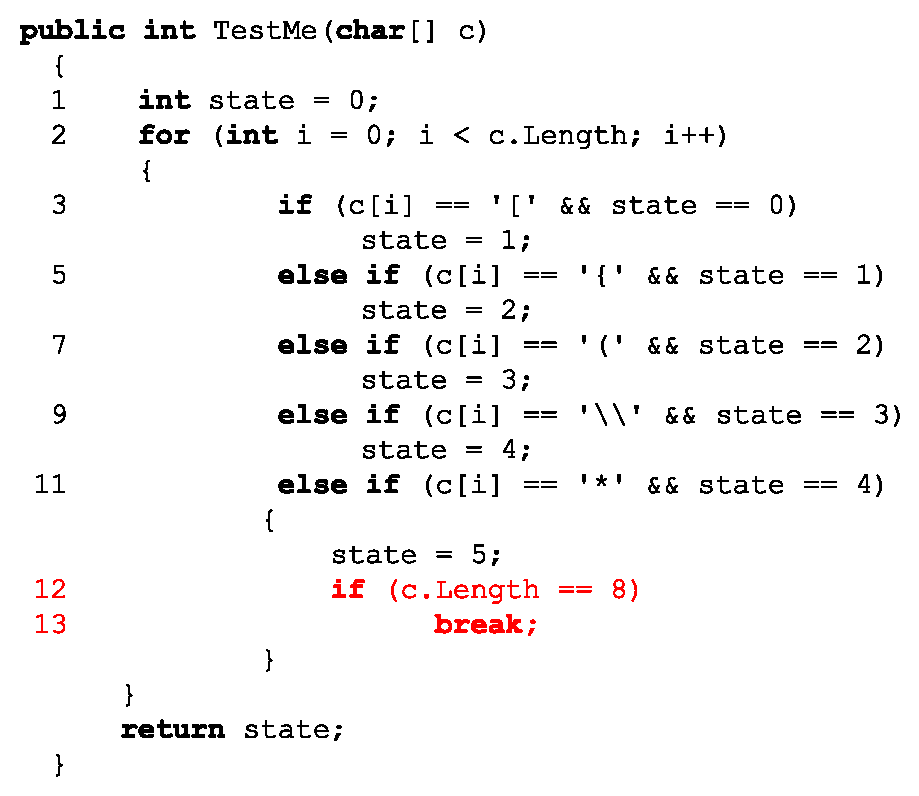
\includegraphics[height=4cm, keepaspectratio]{Figures/ex2}
%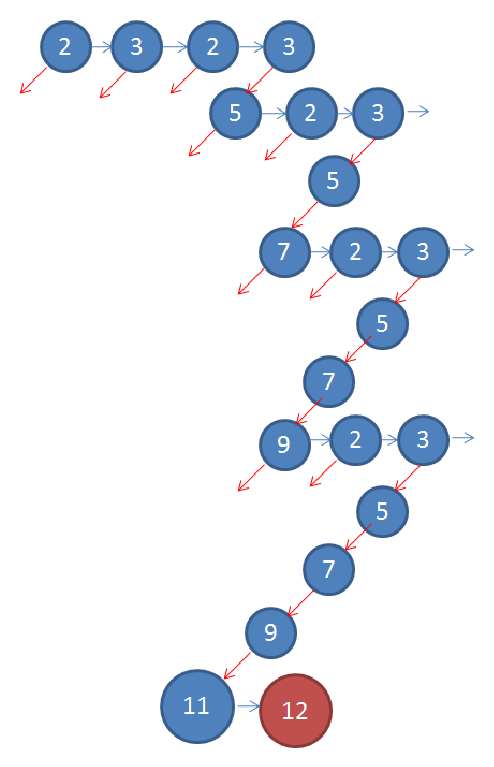
\includegraphics[height=4cm, keepaspectratio]{Figures/exTree}
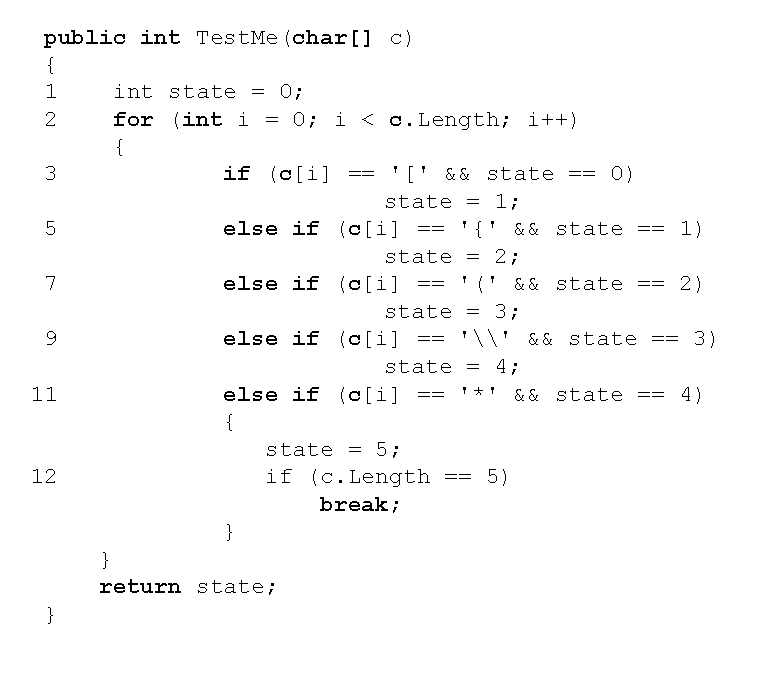
\includegraphics[height=4.7cm, keepaspectratio]{Figures/Presentation3}
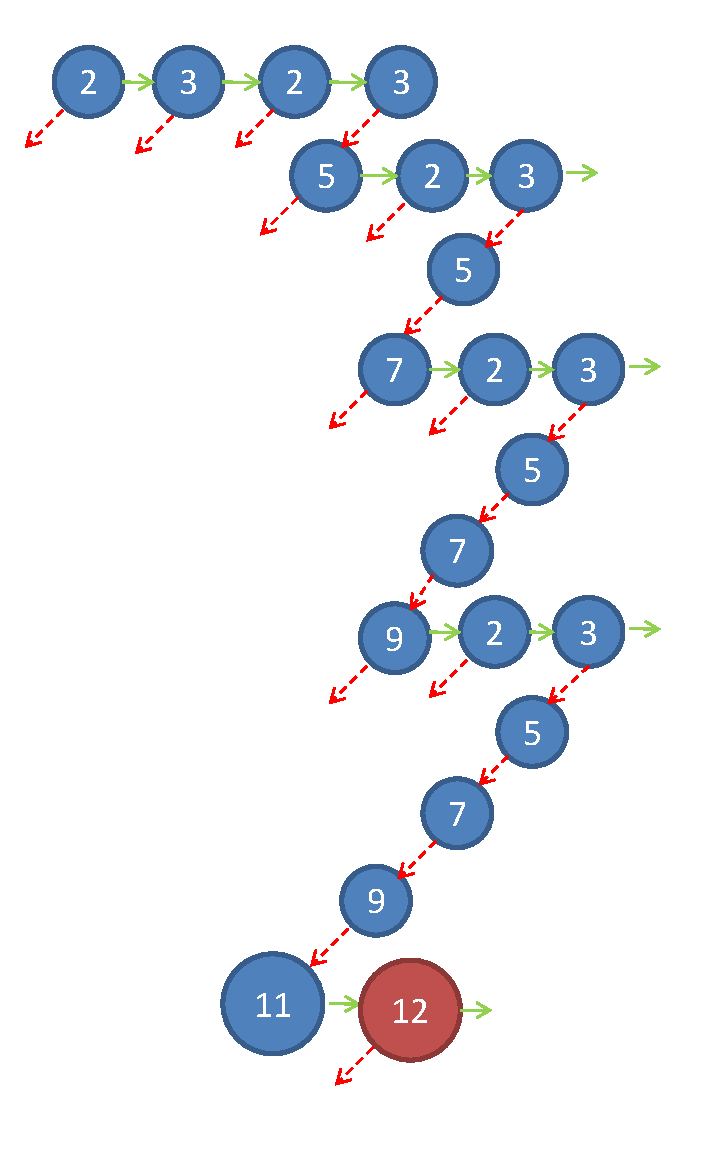
\includegraphics[height=4.7cm, keepaspectratio]{Figures/Presentation2}
\vspace{-0.2 in}
\scriptsize\caption{An example program on the left side with a part of its execution tree for c = \{[, \{, (, $\backslash$, * \} on the right side.}
\vspace{-0.2 in}
\label{fig:example2}
\end{figure}
Let there be an existing test suite covering all the blocks in the old version of the program. Suppose that the test suite has a test input $I$ = \{"[", "\{", "(", "$\backslash$", "*" \}. The input covers all the blocks in the new version of \CodeIn{TestMe} except the newly added block at Line 13. If we start the program exploration from scratch (i.e default input), Pex takes 441 runs to cover the block at Line 13. However, we can reuse the existing test suite for exploration to cover the new block efficiently. Our approach executes the test suite to build an execution tree for the tests in the test suite. Our approach then starts the program exploration using the dynamic execution tree discovered by executing the existing test suite instead of starting from an empty tree. Some of the branches in the tree might take many runs for Pex to discover. The right side of Figure~\ref{fig:example2} shows the part of the execution tree for the input $I$. The red (dotted) edges in the tree indicate false side of the source branching node while the blue (solid) edges indicate the true side. To generate an input for the next DSE run, Pex flips a branching node $b$ in the tree whose the other side has not yet been explored and generates an input so that program execution takes the unexplored branch of $b$. Pex chooses such branch for flipping using various heuristics for covering new parts of the program. Its likely that Pex chooses the branching node 12 (colored red), which on execution covers the block at Line 12. When starting the program exploration from scratch, Pex takes 420 runs before it could discover the red branching node in Figure~\ref{fig:example2}. Using our approach of seeding the tests from the existing test suite, Pex takes 39 runs to flip the branching node and cover the block at Line 12. 